\documentclass{standalone}
\usepackage{tikz}

\begin{document}

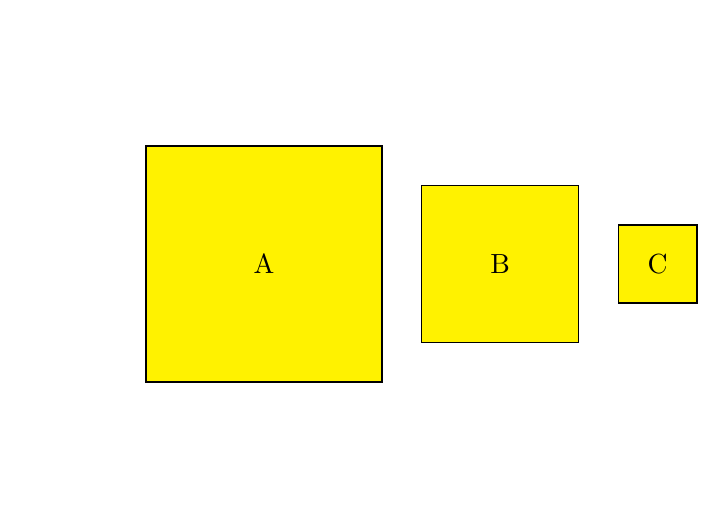
\begin{tikzpicture}
    % Step 1: Draw the white background
    \fill[white] (-3,-3) rectangle (5,3);
    
    % Step 2: Define Node A (largest, 3cm)
    \node[draw, fill=yellow, minimum size=3cm, 
          path picture={
              \draw[black, thick] (path picture bounding box.south west) 
              rectangle (path picture bounding box.north east);
          }] at (0,0) {A};
    
    % Step 2: Define Node B (medium, 2cm)
    \node[draw, fill=yellow, minimum size=2cm, 
          path picture={
              \draw[black, thick] (path picture bounding box.south west) 
              rectangle (path picture bounding box.north east);
          }] at (3,0) {B};
    
    % Step 2: Define Node C (smallest, 1cm)
    \node[draw, fill=yellow, minimum size=1cm, 
          path picture={
              \draw[black, thick] (path picture bounding box.south west) 
              rectangle (path picture bounding box.north east);
          }] at (5,0) {C};
\end{tikzpicture}

\end{document}